\addcontentsline{toc}{subsection}{Extreme Values of Functions}
\subsection*{Extreme Values of Functions}
Extreme values help us answer questions like, \textit{What is the most effective dose of medicine?}, \textit{What is the least expensive way to pipe oil from an offshore refinery down the coast?}\\
\\
\\

\textbf{Absolute} (or global) maximum and minimums means there is no greater/lesser value for $f(x)$ anywhere.\\
\\
\textbf{Local} maximum and minimum means there is no greater/lesser value for $f(x)$ nearby.\\
\\
\textbf{Domain Matters!} Given that $\displaystyle f(x)=\frac{1}{3}x^3-x^2$, find the absolute extrema and the local extrema on the following intervals:

\begin{minipage}[t]{.65\linewidth}
    \hspace{\stretch{8}} local max \hspace{\stretch{1}} abs max \hspace{\stretch{1}} local min \hspace{\stretch{1}} abs min\\
    
    \begin{questions}
        \question $\displaystyle(-\infty,\,\infty)$\\\\
        
        \question $\displaystyle[-3,\,6]$\\\\
        
        \question $\displaystyle(0,\,6]$\\\\
        
        \question $\displaystyle[-3,\,-1]$\\
    \end{questions}
\end{minipage}
\hfill
\begin{minipage}[t]{.25\linewidth}
    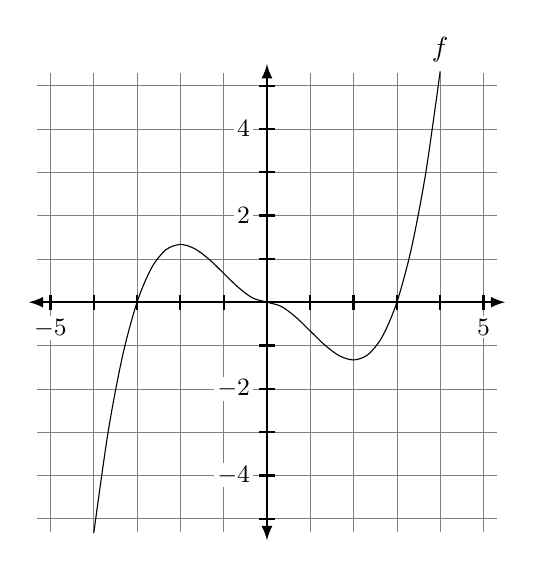
\begin{tikzpicture}[xscale=.55,yscale=.55,baseline=(current bounding box.north)]
        \draw[step=1,style=help lines,] (-5.3,-5.3) grid (5.3,5.3);
        \draw[latex-latex, thick] (-5.5,0)--(5.5,0);
        \draw[latex-latex, thick] (0,-5.5)--(0,5.5);
        \foreach \x in {-5,5}
            \draw[thick] (\x,5pt) -- (\x,-5pt) node [below=.7mm,fill=white,inner sep=1pt] {\small$\x$};
        \foreach \y in {-2,2,-4,4}
            \draw[thick] (5pt,\y) -- (-5pt,\y) node [left=.7mm,fill=white,inner sep=1pt] {\small$\y$};
        \foreach \x in {-3,-1,1,3,2,-2,4,-4}
            \draw[thick] (\x,5pt) -- (\x,-5pt);
        \foreach \y in {1,-1,3,-3,5,-5}
            \draw[thick] (5pt,\y) -- (-5pt,\y);
            
        \draw[] plot[smooth, domain=-4:4] (\x, {(1/3)*(\x^(3))-(\x^(2))}) node[anchor=south] {$f$};
    \end{tikzpicture}
    
\end{minipage}
\vspace{1cm}

\begin{tcolorbox}[title= THE EXTREME VALUE THEOREM,colframe=black,sharp corners,colback=white,colbacktitle=white,coltitle=black,boxrule=1pt]

    If $f(x)$ is continuous on the closed interval $[a,\,b]$, then $f(x)$ has both a maximum value and a minimum value on the interval.
    
\end{tcolorbox}
\vspace{1cm}
Naturally the question becomes: \textbf{How can we find the extreme values?} \underline{\hspace{3cm}}!!!!


\newpage


\begin{tcolorbox}[title= DEFINITION OF LOCAL EXTREME VALUES,colframe=black,sharp corners,colback=white,colbacktitle=white,coltitle=black,boxrule=1pt]

    If a function $f(x)$ has a local maximum or minimum value at an interior point $c$ of its domain, and if $f'(x)$ exists at $c$, then $f'(c)=0$. 
    
\end{tcolorbox}
\vspace{1cm}
But sometimes a maximum or a minimum may occur when $f'(c)\ne0$. What might cause this to happen?
\begin{center}
    \underline{\hspace{6cm}}
\end{center}
\vspace{2cm}

Instead, lets introduce a definition that encompasses ALL these points:\\

\begin{tcolorbox}[title= DEFINITION OF A CRITICAL POINT,colframe=black,sharp corners,colback=white,colbacktitle=white,coltitle=black,boxrule=1pt]

    Let $f$ be defined at $c$. If $f'(c)=0$ or if $f$ is not differentiable at $c$, then $c$ is a \textbf{critical point} (or \textbf{critical number}) of $f$.\\
    \\
    As a consequence, \textbf{relative extrema only occur at critical points!}
    
\end{tcolorbox}
\vspace{.15cm}
\noindent\textbf{Example:}\\
Find the extrema of $f(x)=3x^4-4x^3$ on the interval $[1,\,2]$.

\newpage

\noindent\textbf{More Examples:}
\begin{questions}
    \question Find the absolute maximum and minimum values of $f(x)=x^{2/3}$ on the interval $[-2,\,3]$.
    \vspace{\stretch{1}}
    
    \question Find the extreme values of  $\displaystyle f(x)=\frac{1}{\sqrt{4-x^2}}$.
    \vspace{\stretch{1}}
    
    \question Find the extreme values of $\displaystyle f(x)=\begin{cases}
    5-2x^2 & x\le1\\ x+2 & x>1
    \end{cases}$.
    \vspace{\stretch{1}}
    
    \question Find the extreme values of $\displaystyle f(x)=\ln\left|\frac{x}{1+x^2}\right|$.
    \vspace{\stretch{1}}
    
    \question Let $f(x)=|x^3-9x|$
        \begin{parts}
            \part Does $f'(0)$ exist?
            \part Does $f'(3)$ exist?
            \part Does $f'(-3)$ exist?
            \part Determine all extrema of $f(x)$.
        \end{parts}
\end{questions}

\newpage

\begin{tcolorbox}[title= THE FIRST DERIVATIVE TEST,colframe=black,sharp corners,colback=white,colbacktitle=white,coltitle=black,boxrule=1pt]

    The following applies to a continuous function $f(x)$.
    \begin{questions}
        \question If $f'(x)$ changes sign from positive to negative at a critical point $c$, then $f(x)$ has a local maximum value at $c$.
        \question If $f'(x)$ changes sign from negative to positive at a critical point $c$, then $f(x)$ has a local minimum value at $c$.
        \question If $f'(x)$ does not change sign at a critical point $c$, then $f(x)$ has no local extreme value at $c$.
    \end{questions}
    
    
\end{tcolorbox}
\vspace{.15cm}
\textbf{Examples:} Identify any local extrema using the first derivative test. Then identify any absolute extrema.
\begin{questions}
    \begin{minipage}{.45\linewidth}
        \question $\displaystyle f(x)=x^2-12x-5$
    \end{minipage}
    \hfill
    \begin{minipage}{.45\linewidth}
        \question $\displaystyle g(x)=\left(x^2-3\right)e^x$
    \end{minipage}
\end{questions}

\vspace{\stretch{1}}

There are times when a curve can hold water or spill water. We call this ability \textbf{concavity}.\\

\begin{tcolorbox}[title= THE CONCAVITY TEST,colframe=black,sharp corners,colback=white,colbacktitle=white,coltitle=black,boxrule=1pt]
    The graph of a twice differentiable function $f(x)$ is
    \begin{questions}
        \question concave up if $f''(x)>0$.
        \question concave down if $f''(x)<0$.
    \end{questions}
    
    The point where the graph has a tangent line and when the concavity changes is a \textbf{point of inflection}. When $f''(x)=0$ or $f''(x)$ DNE are both candidates for POI's.
    
\end{tcolorbox}


\newpage


\begin{tcolorbox}[title= THE SECOND DERIVATIVE TEST,colframe=black,sharp corners,colback=white,colbacktitle=white,coltitle=black,boxrule=1pt]

    \begin{questions}
        \question If $f'(c)=0$ and $f''(c)<0$, then $f(x)$ has a local maximum at $x=c$.
        \question If $f'(c)=0$ and $f''(c)>0$, then $f(x)$ has a local minimum at $x=c$.
    \end{questions}
    
    The test fails if $f''(c)=0$ or if $f''(c)$ does not exist.
    
\end{tcolorbox}

\textbf{Examples:} Find the local extreme values of the following.
\begin{questions}
    \begin{minipage}{.45\linewidth}
        \question $y=x^4$
    \end{minipage}
    \hfill
    \begin{minipage}{.45\linewidth}
        \question $f(x)=\sqrt[3]{x}$
    \end{minipage}

    \vspace{\stretch{1}}
\end{questions}

